\documentclass{report}

\input{~/dev/latex/template/preamble.tex}
\input{~/dev/latex/template/macros.tex}

\title{\Huge{}}
\author{\huge{Nathan Warner}}
\date{\huge{}}
\pagestyle{fancy}
\fancyhf{}
\lhead{Warner \thepage}
\rhead{}
% \lhead{\leftmark}
\cfoot{\thepage}
\setborder
% \usepackage[default]{sourcecodepro}
% \usepackage[T1]{fontenc}

\begin{document}
    % \maketitle
        \begin{titlepage}
       \begin{center}
           \vspace*{1cm}
    
           \textbf{Discrete Structures}
    
           \vspace{0.5cm}
           Notes
            
                
           \vspace{1.5cm}
            A document by: \\ 
           \textbf{Nathan Warner}
    
           \vfill
                
                
           \vspace{0.8cm}
         
           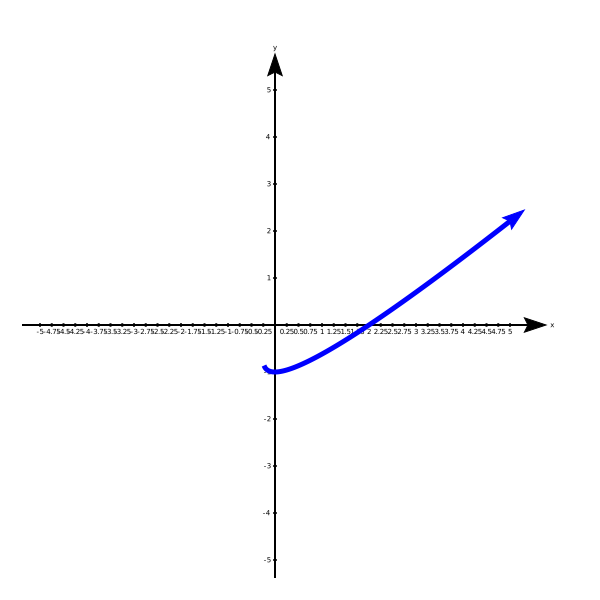
\includegraphics[width=0.4\textwidth]{./figures/1.png}
                
           Computer Science \\
           Northern Illinois University\\
           United States\\
           
                
       \end{center}
    \end{titlepage}
    \tableofcontents
    \pagebreak 
    \begin{center}
        \section{Set Theory}
    \end{center}
    \line(1,0){490}
    \bigbreak \noindent 
    \subsection{Definition of a set} 
    \bigbreak \noindent 
    \begin{mdframed}
        \textbf{Definition:} A \textbf{set} is a collection of elements 
        \smallbreak \noindent
        We denote sets with the following syntax:
        \begin{align*}
            A  = \{1,2,3,4\}
        .\end{align*}
        Where in this case $A$ is the identifier and it's elements are delimited by commas and encapsulated among braces.
        \smallbreak \noindent
        \textbf{Note:} The identifier for sets are commonly represented with capital letters
        \bigbreak \noindent 
        We can also indicate \textit{infinitely many} elements in a set by use of the \textbf{ellipsis}, which would look like:
        \begin{align*}
            A = \{1,2,3,...\} \\
            Generally:\ A=\{A_{1}, A_{2}, A_{3},...,A_{n}\}
        .\end{align*}
    \end{mdframed}
    \bigbreak \noindent 
    \textbf{More Notation:}
    We can indicate that an object is an \textbf{element} of a set with the following syntax:
    \begin{align*}
        A = \{1,2,3,4\} \\
        3 \in A
    .\end{align*}
    \bigbreak \noindent 
    \subsection{Number Sets}
    \bigbreak \noindent 
    The set of \textbf{Natural Numbers} (whole numbers) is denoted by $\mathbb{N}$:
    \begin{align*}
        \mathbb{N}: 1,2,3,..
    .\end{align*}
    \bigbreak \noindent 
    The set of \textbf{Integers} is denoted by $\mathbb{Z}$:
    \begin{align*}
        \mathbb{Z}: -5,-4,-3-,2,-1,0,1,2,3,4,5,..
    .\end{align*}
    \bigbreak \noindent 
    So you can see the set of all integers is similar to that of the natural numbers, however this set includes \textit{negative numbers}
    \bigbreak \noindent 
    The set of \textbf{Rational numbers}, (ratio of two integers), is denoted by $\mathbb{Q} $:
    \begin{align*}
        \mathbb{Q}: \frac{1}{6}, \frac{1}{4}, \frac{1}{2},..
    .\end{align*}
    \bigbreak \noindent 
    The set of \textbf{Irrational numbers}, is denoted by $\bar{\mathbb{Q}} $:
    \begin{align*}
        \bar{\mathbb{Q}}: \pi, e, \sqrt{2},\ etc
    .\end{align*}
    \bigbreak \noindent 
    \nt{    for a number to be considered irrational, they cannot be exactly represented as fractions of integers and have non-repeating, non-terminating decimal representations. Thus, the following condition must hold:
    \begin{align*}
        x \text{ is irrational} \iff \frac{a}{b}, \quad \text{where } a \land b \notin \mathbb{Z} \text{ and } \gcd(a, b) = 1.
        % \frac{a}{b}, \quad\ where\ a \land b \notin \mathbb{Z}
    .\end{align*}
}
    \bigbreak \noindent \bigbreak \noindent 
    The set of all \textbf{Real numbers} is denoted by $\mathbb{R}$:
    \begin{align*}
        \mathbb{R}:\ \text{Both rational and irrational numbers}
    .\end{align*}
    \bigbreak \noindent 
    The set of all \textbf{imaginary numbers} is denoted by $\mathbb{I}$:
    \begin{align*}
        \mathbb{I}:\ i^{2} = -1,\ i = \sqrt{-1}\\
        Ex:\ \sqrt{-9} = \sqrt{9} \cdot \sqrt{-1} = 3i
    .\end{align*}
    \bigbreak \noindent 
    The set of \textbf{Complex numbers}, which describes numbers that are comprised of two components, one real and one imaginary, and is denoted by:
    \begin{align*}
        \mathbb{C}: 2+3i
    .\end{align*}
    \bigbreak \noindent 
    \textbf{In summary:}
    \begin{itemize}
        \item $\mathbb{N}$: Denotes the set of all \textbf{Natural Numbers}
        \item $\mathbb{Z}$: Denotes the set of all \textbf{Integers}
        \item $\mathbb{Q}$: Denotes the set of all \textbf{Rational Numbers}
        \item $\mathbb{\bar{Q}}$: Denotes the set of all \textbf{Irrational Numbers}
        \item $\mathbb{I}$: Denotes the set of all \textbf{Imaginary Numbers}
        \item $\mathbb{C}$: Denotes the set of all \textbf{Complex Numbers}
    \end{itemize}
    \bigbreak \noindent 
    \textit{Figure:}
    \begin{figure}[ht]
        \centering
        \incfig{figab}
        \label{fig:figab}
    \end{figure}
    \pagebreak 
    \subsection{Set Equality}
    \bigbreak \noindent 
    \begin{mdframed}
        \textbf{Definition:} An \textbf{axiom} is a rule or statement that is generally accepted to be true without proof.\\
        An \textbf{Axiom of Extension} is a set determined by what its elements are - not the order in which they might be listed or the fact that some elements might be listed more than once.
    \end{mdframed}
    \bigbreak \noindent 
    Consider the sets:
    \begin{align*}
        A = \{1,3,5,1,5,5,3\} \\
        B = \{1,3,5\}
    .\end{align*}
    \bigbreak \noindent 
    Because of the \textbf{Axiom of Extension}, which states that a set is not determined by the order or possible repetitions, we can conclude that $A=B$.
    \bigbreak \noindent 
    Furthermore, we can conclude that we only have $3$ elements amongst set $A$, although it may seem like we have 7.

    \bigbreak \noindent \bigbreak \noindent 
    \subsection{Set-Builder Notation}
    \bigbreak \noindent 
    \textbf{Set-Builder} is a convention we can use when dealing with sets to imply the elements of a set without listing all of its values.
    \bigbreak \noindent 
    Suppose we have:
    \begin{align*}
        x = -5,4,3,-10,-5,2,0
    .\end{align*}
    \bigbreak \noindent 
    Then:
    \begin{align*}
        \{x | x < 0 \}\ \text{Reads: "The set of all x's such that (pipe) x is less than zero"} \\
        = \{-10,-5\}
    .\end{align*}
    \bigbreak \noindent 
    So naturally you can infer that this set would be all x's from are defined pool of x values that are negative. 
    \bigbreak \noindent 
    Additionally, we can utilize \textit{Number Sets}:
    \begin{align*}
        \{x \in \mathbb{R} | -2 < x < 5\}
    .\end{align*}

    \bigbreak \noindent \bigbreak \noindent 
    \subsection{Types of Sets}
    \bigbreak \noindent 
    \begin{itemize}
        \item \textbf{Universal Set}: Denoted $\mathbb{U}$, represents the collection of all possible elements or objects that are under consideration for a particular context or problem.
        \item \textbf{Empty Set (Null set)}: Denoted $\emptyset$ (phi), represents a set that contains no elements
        \item \textbf{Singleton Set}: Represents a set that only has one element
        \item \textbf{Finite Set}: Represents a set that has a countable number of elements
        \item \textbf{Infinite Set}: Represents a set that has an infinite amount of elements
        \item \textbf{Subset}: A set in which all elements are part of a larger set 
    \end{itemize}
    \bigbreak \noindent 
    \begin{mdframed}
        \textbf{Definition:} \textbf{Cardinal Number of a Set:} is the number of elements in a set, denoted $n(A)$. Where, in this case, $A$ represents the name of the set.
    \end{mdframed}
    \bigbreak \noindent 
    Consider the set:
    \begin{align*}
        A = \{1,2,3\} \\
        Then:\ n(A) = 3
    .\end{align*}
    \bigbreak \noindent 
    Where $n(A) = 3$ represents the cardinal number of the set
    \bigbreak \noindent 
    \begin{mdframed}
        \textbf{Definition:} \textbf{Equivalent Set:} Represents sets that have the same \textit{Cardinal Number}. To show that two sets are equivalent, we can use the notation:
        \begin{align*}
            A \sim B 
        .\end{align*}
        \bigbreak \noindent 
        Which shows that the cardinality of $A$ equals the cardinality of $B $ 
    \end{mdframed}
    \bigbreak \noindent 
    Consider the sets:
    \begin{align*}
        A = \{1,4,5\} \\
        B = \{6,8,10\}
    .\end{align*}
    \bigbreak \noindent 
    Then we can say:
    \begin{align*}
        A \sim B 
    .\end{align*}
    



    
\end{document}
